\subsection{Preparation: improving the starting point of on-policy learning}
\label{sec:source}
\label{sec:reachability}
\label{sec:preparation}

\begin{figure}[!h]
%\vspace{-1em}
\centering
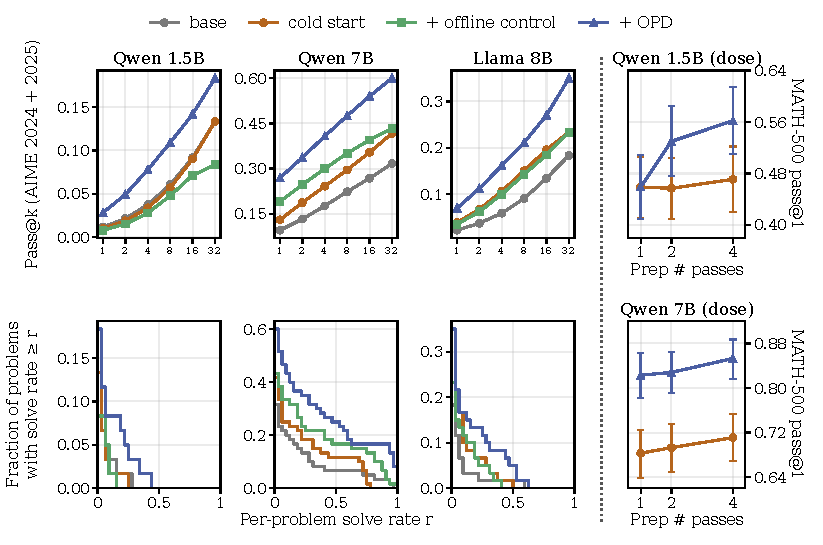
\includegraphics[width=1.0\linewidth]{figures/fig_combined_aime_dose.pdf}
\caption{\textbf{Offline-prepared OPD improves sampled coverage and reliability.} Left: pooled AIME 2024/2025 pass@$k$ for $k\le32$ (top) and the fraction of problems with empirical solve rate $\ge r>0$ (bottom), using 32 responses per problem from batch~a. Right: preparation dose versus strict MATH-500 pass@1, using the step-100 OPD checkpoint at 1.5B and the best evaluated checkpoint within 100 steps at 7B; error bars are 95\% problem-bootstrap intervals. See \cref{app:preparation-multisetup,app:preparation-legacy} for protocols and paired comparisons.}
\label{fig:preparation-aime}
\end{figure}

\Cref{sec:broadcast} suggests a direct intervention. As we saw in the last sub-section, OPD can fail because early policy changes route the weak student model into reasoning states it cannot yet execute reliably, and the training run spends a large chunk of time fitting unreliable requests on increasingly lower-quality prefixes. Then, a natural candidate intervention is that, before OPD, we force the student to visit higher-quality prefixes from the teacher itself and learn the teacher's stronger continuations on those prefix populations. This suggests offline distillation to prepare the student model's continuation abilities before running OPD, which can then expose finer student errors to the teacher and sustain more stable learning trajectory for online corrections when OPD changes prefix visitation, without the requests looking so foreign to the student in the OPD phase that it routes into irrecoverable rollout distributions.
%It may therefore improve continuation skills and reasoning-state management that become useful as OPD changes visitation. This motivates a cold start \citep{rethinking_opd_2026} as preparation for subsequent on-policy learning.

We prepare with student/teacher pairings Qwen2.5-1.5B-Instruct/JustRL-1.5B \citep{qwen2025qwen25technicalreport,he2025justrlscaling15bllm}, Qwen2.5-7B-Instruct/AceReason-Nemotron-7B \citep{liu2025acereasonnemotron11advancingmath}, and Llama-3.1-8B-Instruct/Llama-3.1-Nemotron-Nano-8B-v1 \citep{grattafiori2024llama3herdmodels,bercovich2025llamanemotronefficientreasoningmodels}, with students trained on their teachers' solutions to OpenMathInstruct-2 \citep{toshniwal2024openmathinstruct2}. We then compare OPD with continued offline distillation on the same DAPO-Math-17k prompt blocks \citep{yu2025dapo}, matching optimizer steps and sequence presentations. 



\Cref{fig:preparation-aime} shows higher pooled pass@$k$ accuracy for OPD than offline training through $k=32$, using 32 responses per problem. The gains extend beyond pass@1 to sampled coverage and the distribution of per-problem solve rates. The \emph{reliability} improvement is especially interesting: looking at pass@$k$ alone might give us the impression that OPD just solves more problems by rare chances, however, we find that OPD with appropriate preparation also enhances the per-problem solve rates for the models beyond the offline-distillation-only alternatives. Additionally, the preparation ``dose study'' (\cref{fig:preparation-aime}, right) shows increasing value of offline-preparation for the later OPD phase. At 1.5B, one to four passes leaves the starting strict MATH pass@1 at $45.7$--$47.1\%$, but raises the 100-step OPD endpoint from $45.9\%$ to $56.2\%$. Similar trends are observed at 7B (\cref{app:preparation-legacy}). Please refer to \cref{app:preparation-multisetup} for further details.

